
\section{Analisi dei dati}
\subsection{Scarto quadratico medio}
    Dopo aver preso le misure sulle velocità delle gocce d'olio siamo riusciti a risalire tramite l'equazione \eqref{raggio} ai raggi delle goccioline d'olio.\\
    Ottenuto il raggio, è bastato inserirlo nelle equazioni \eqref{caricapos}, \eqref{caricaneg} per stimare le cariche sulle goccioline d'olio.\\
    A questo punto dell'analisi, ottenute tutte le cariche delle gocce, abbiamo potuto condurre un'indagine statistica per individuare quale valore \textit{q} approssimasse al meglio una quantità che, dividendo la carica \textit{Q} totale della goccia, restituisse un numero intero.\\
    Abbiamo potuto svolgere questa indagine sotto l'ipotesi che la carica elettrica fondamentale, quella dell'elettrone, fosse quantizzata.\\
    Abbiamo considerato $\{q_\alpha\}_{\alpha=1,2,\dots,M}$ cariche che abbiamo chiamato di \textit{prova}.\\
    La scelta di queste è arbitraria e noi le abbiamo stabilite dividendo l'intervallo $\left[1.45,1.9\right]\cdot10^{-19}~C$ in M $=400$ sottointervalli, i quali estremi erano proprio le $\{q_\alpha\}_{\alpha=1,2,\dots,M}$.
    Abbiamo poi definito la funzione 
        $$S(q_\alpha)=\sum_{k=1}^{N_{misure}} \left( \frac{Q_i}{k_i(q_\alpha)} - q_\alpha\right) ~~con~~ k_i(q_\alpha)=\left\lfloor \frac{Q_i}{q_\alpha + 0.5} \right\rfloor$$
    detta \textit{scarto quadratico medio}, utile per determinare quanto la carica n-esima di prova si discostasse dal quantificare la carica quantizzata elementare.\\
    Il valore di $q_alpha$ che minimizza questa funzione di loss coincide con il valore della carica elettrica dell'elettrone.
    Minimizzando la funzione $S(q_\alpha)$, si trova che il suo minimo coincide con la quantità:
        $$q_{vero}=\frac{1}{N_{misure}}\cdot \sum_{i=1}^{N_{misure}} \frac{Q_i}{k_i}$$
    Abbiamo infine assegnato alla misura un errore che corrispondesse alla deviazione standard della media:
        $$\sigma_{\overline{q}} = \sqrt{\frac{S(\overline{q})}{N \cdot (N-1)}} ~~con~~ N=N_{misure}$$

    \subsection{Grafico ricerca carica elettrone}
\begin{figure}[H]
    \centering
    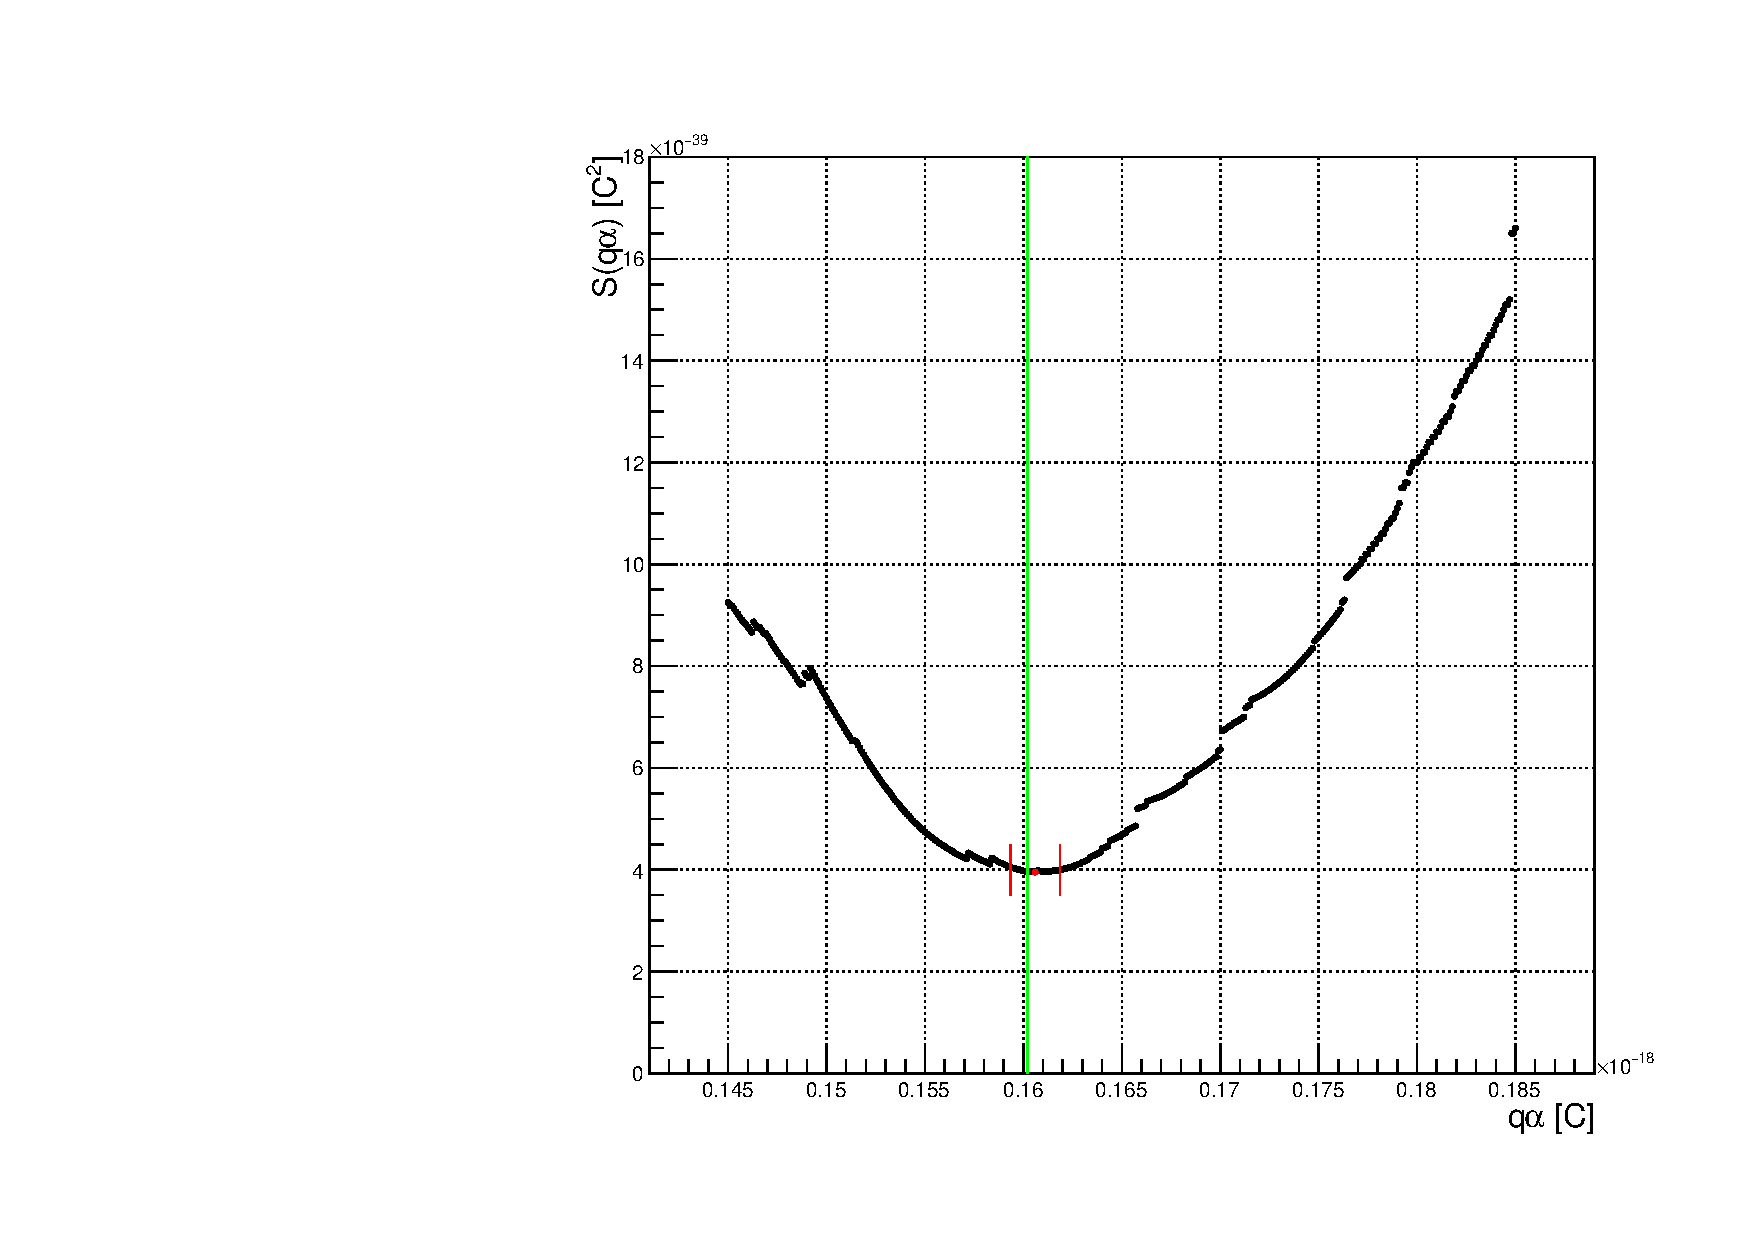
\includegraphics[width=\textwidth,height=\textheight,keepaspectratio]{graph1.pdf}
    \caption{Grafico di S(q$\alpha$), con ricerca carica minima}
\end{figure}
    
\subsection{Rigetto dei dati}
Un aspetto importante che abbiamo tenuto conto nell'analizzare i dati sperimentali è che la procedura con cui sono stati misurati i tempi era affetta principalmente da 2 fonti di errore:\begin{itemize}
    \item tempo di reazione umano a stimolo uditivo e utilizzo del cronometro;
    \item il moto delle gocce in determinate situazioni non era completamente uniforme, rendendo difficile determinare quando esse attraversavano la linea spessa della griglia.
\end{itemize}
Abbiamo quindi scelto di calcolare la media delle cariche sperimentali misurate per ogni goccia (con entrambe le configurazioni di campo elettrico) e a quel punto calcolare in percentuale quanto il dato sperimentale si discostasse dalla media.
Poiché idealmente la carica totale della goccia non dovrebbe modificarsi durante il moto (a meno di acquisto/perdita di 1 elettrone) abbiamo scelto di scartare tutte le misure che avevano uno scarto maggiore del 5\% rispetto al valore medio.\\
Nell'analisi statistica la media è considerata quella pesata, in quanto ad ogni carica sperimentale è associata un'incertezza.\\